\chapter{Bispecific T-cell engagers}
\label{chap:immune}

Bispecific T cell engagers have proven to be a potent antibody design in cancer immuno-oncology by forming a trinary complex when binding to an immune cell and a cancer cell simultaneously.
This type of antibody substitutes the role of antigen presenting cells to activate the immune cells against the cancer cells. 
T cell engagers should be carefully designed to have maximum potency, the immune cell-antibody-cancer cell trinary complex concentration, against tumor cells and circumvent cytokine storm in the body.
A relatively high concentration of the antibody, increases the risk of cytokine storm, saturates the number of immune cell-antibody and antibody-cancer cell dimers, and hinders a potent response.
A low concentration of the antibody is not sufficient to produce a potent concentration of trinary complex to activate the immune system against the cancer cells.
The purpose of this study is to quantitatively investigate how the concentration of trinary complex, and distribution are dependent on the design characteristics of the bispecific antibodies, like the binding kinetics to the target receptors on the immune cells and the cancer cells.
Several antibodies that are either clinically approved, or currently under clinical/preclinical development process are simulated to explore if the kinetics can be enhanced with a different design.
Moreover, the identifiability analysis done in this work proves the sufficiency of steady state data for identifiability of the dissociation rates.

\section{Introduction}

\ac{BiTE} has shown an strong cancer immunotherapy strategy in recent years~\cite{stieglmaier2015utilizing, yuraszeck2017translation, betts2020mechanistic, tian2021bispecific}. \ac{BiTE} technology has been proposed for treating acute myeloid leukemia~\cite{laszlo2014cellular}, multiple myeloma~\cite{hipp2017novel}, lymphoblastic leukemia~\cite{topp2014phase}, refractory solid tumors~\cite{kebenko2018multicenter}, and as a platform for targeted therapy across different tumor types~\cite{einsele2020bite}. A list of \ac{BiTE} molecules that were considered in this study is presented in table~\ref{table:bites}. This list is made by selecting the \ac{BiTE} molecules that their binding kinetics to the targets were specified in the literature. More detailed review of the existing \ac{BiTE}s or bispecific antibodies has been recently done recently by~\cite{gera2022evolution, tian2021bispecific, morcos2021quantitative}.

The targeted receptor protein of cancer cells are biomarkers of the cancer cells that have minimal expression in normal cells to have minimum off target effects. Also, \ac{BiTE}s might have different chemical structure formats with different number of binding sites. The targeted receptor protein of immune cell is CD3 receptor of T cells for all the \ac{BiTE}s considered in this study.

A three-body model~\cite{douglass2013comprehensive} is what all bispecific antibodies have in common. In the three-body model a bispecific antibody, binding species, connects to two different target molecules, terminal species, to form a trinary complex. After the formation of dimers of the first target and the anibody, the binding kinetics can be changed based on Cooperativity factor to increase/decrease the binding affinity of the antibody molecule of the formed dimer to the second target. A positive Cooperativity factor increases the binding affinity, and it can be interpreted as the avidity factor explained in the bispecific antibody literature~\cite{rhoden2016modeling, sengers2016modeling, harms2014understanding, kaufman1992effect}, where the bispecific antibody is targeting two different receptors of the same cell type for an increased specificity. The Cooperativity factor can be neglected in models of bispecific antibodies that are targeting two different cell types like~\ac{BiTE}, as the dimers are free in the spatial coordinates to bind to the second target. In this study, the first objective is to evaluate the design characteristics of \ac{BiTE}s based on the simple model presented in figure~\ref{fig:three-body}. The~\ac{BiTE} antibody, $X$, is targeting receptors on the immune cells, $T_1$ which usually is the CD3 receptor of T cells, and the protein receptor of cancer cells, $T_2$.  

\begin{figure}[!hb]
	\centering
	\begin{subfigure}[b]{0.66\textwidth}
		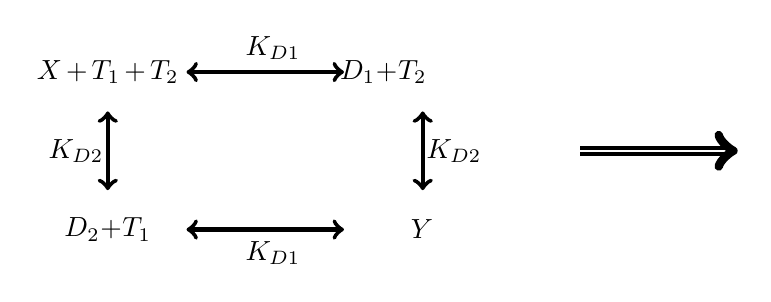
\begin{tikzpicture}
			\node[text width=1.8cm] at (-1,1.5) {$X+T_1+T_2$};
			\node[text width=1.1cm] at (+2.5,1.5) {$D_1+T_2$};
			\node[text width=1.1cm] at (-1,-0.5) {$D_2+T_1$};
			\node[text width=0.3cm] at (+3,-0.5) {$Y$};
			\draw[ultra thick, <->] (-1,0) -- (-1,1);
			\draw[ultra thick, <->] (3,0) -- (3,1);
			\draw[ultra thick, <->] (0,-0.5) -- (2,-0.5);
			\draw[ultra thick, <->] (0,1.5) -- (2,1.5);
			\node[text width=0.5cm] at (+1,+1.8) {$K_{D1}$};
			\node[text width=0.5cm] at (+1,-0.8) {$K_{D1}$};
			\node[text width=0.5cm] at (-1.5,0.5) {$K_{D2}$};
			\node[text width=0.5cm] at (+3.3,0.5) {$K_{D2}$};
			\draw[ultra thick, double, ->] (5,0.5) -- (7,0.5);
		\end{tikzpicture}\\
		\begin{minipage}{1cm}
			\vfill
		\end{minipage}
	\end{subfigure} 
	\begin{subfigure}[b]{0.33\textwidth}
		\centering
		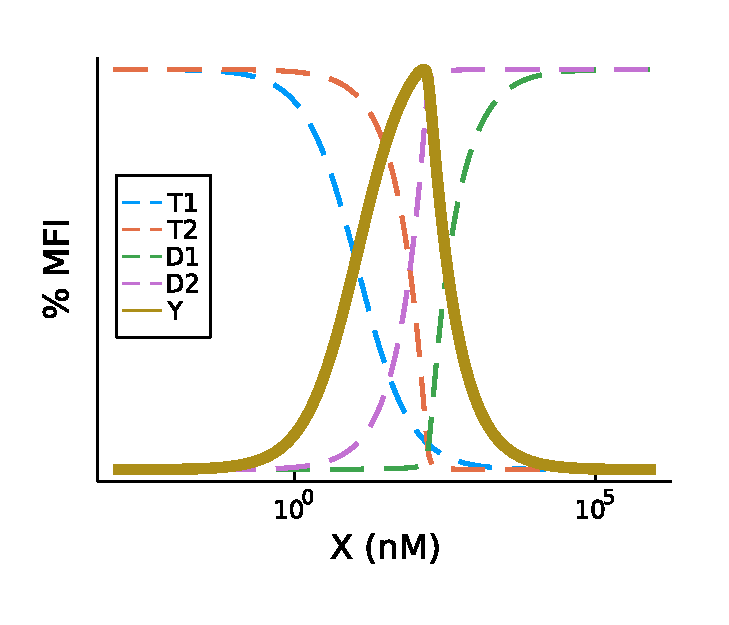
\includegraphics[width=1\textwidth]{fig/bell-shape.pdf}
	\end{subfigure}
	\caption[Three-body model]{On the left side, the three-body model of \ac{BiTE}, $X$, $T_1$ and $T_2$ are the two target receptors on immune and cancer cells, $D_1$ and $D_2$ are the dimers of bispecific antibody-immune cell and bispecific antibody-cancer cell, $Y$ is the trimer complex, and $k_{D1}$ and $k_{D2}$ are the dissociation constants of the antibody binding equilibrium. The chemical reactions are visualized in a simple form to provide an intuitive idea of the reactions, specifically $T_2$ ($T_1$) is not involved in dimerization reaction between $X$ and $T_1$($T_2$), i.e. the differential equations presented in~\eqref{eq:three-body} do not follow mass-action kinetics from the visualized chemical reaction network. On the right side, a nominal bell-shape pattern of the trinary complex $Y$ in fluorescent intensity is visualized as a function of \ac{BiTE} concentration. Binding kinetics and initial conditions are adopted from~\cite{betts2019translational}. }
	\label{fig:three-body}
\end{figure}

\begin{landscape}
\begin{table}[ht]
	\centering
	\caption[\ac{BiTE} molecules]{CD3 \ac{BiTE}s (sorted by the year of the referenced publication)}
	\begin{tabular}{l l c c c c c r} 
		\hline \vspace{-7pt}\\
		CD3 \ac{BiTE} & Target & $k_{D1}$(nM) & $k_{D2}$(nM) & Type & Format & kDa & Ref \\ [0.5ex] 
		\hline \vspace{-7pt}\\
		Blinatumomab & CD19 & $\sim 100$ & $\sim 1$  & Liquid & BiTE & 54 & \cite{dreier2002extremely}  \\
		Solitomab & Ep-CAM & $16\pm12$ & $77\pm39$ & Liquid & BiTE & 55 & \cite{brischwein2006mt110}  \\
		BAY2010112 & PSMA & $9.4\pm4.3$ & $47.0\pm8.1$ & Solid & BiTE & 55 & \cite{friedrich2012regression} \\
		PF-06671008 & Pcad & $11.5\pm0.9$ & $0.521\pm0.162$ & Solid & DART & 57 & \cite{root2016development}  \\
		CD3$_\varepsilon$L/HER2 & HER2 & $50$ & $0.5$ & Solid & KIH & $>100$ & \cite{mandikian2018relative}  \\
		CD3$_\varepsilon$H/HER2 & HER2 & $0.5$ & $0.5$ & Solid & KIH & $>100$ & \cite{mandikian2018relative}  \\
		CD3$_\varepsilon$VH/HER2 & HER2 & $0.05$ & $0.5$ & Solid & KIH & $>100$ & \cite{mandikian2018relative}  \\
		7370 & FLT3 & $27$ & $49\times10^{-3}$ & Liquid & IgG-based & 146 & \cite{yeung2020optimized}  \\
		PF-07062119 & GUCY2C & $7.47\pm0.15$ & $23.97\pm0.97$ & Solid & IgG1-FcyR & $>100$ & \cite{mathur2020novel}  \\
		Tarlatamab & DLL3 & $0.64\pm0.05$ & $14.9\pm0.4$ & Solid & HLE-BiTE & $>100$ & \cite{giffin2021amg} \\
		Acapatamab & PSMA & $22.4\pm2.8$ & $14.8\pm2$ & Solid & HLE-BiTE & $>100$ & \cite{deegen2021psma} \\
		Anti-CD79b/CD3 & CD79b & $12.8$ & $1$ & Liquid & KIH & $150$ & \cite{yadav2022nonclinical} \\
		\hline
	\end{tabular}
	\label{table:bites}
\end{table}
\end{landscape}

In the recent investigations such as \cite{betts2019translational,douglass2013comprehensive} it has been emphasised that the efficacy of \ac{BiTE}, trimer concentration at the cite of action, is a bell-shape function. A relatively low or high concentration of a \ac{BiTE} is not effective to produce enough number of trimer complexes to activate the immune cells against the cancer cells. At a low concentration the \ac{BiTE} concentration is simply not enough to produce a potent concentration of trimer complex $Y$. At a high concentration the \ac{BiTE} saturates the target receptor proteins on the immune cells and cancer cells, in a way that the dimers of immune cell - \ac{BiTE}, $D_1$, and \ac{BiTE} - cancer cell, $D_2$, increase and limit the number of free targets to form the trinary complex $Y$. 
Besides that, a high concentration of the \ac{BiTE} can potentially cause off target side effects in the body or end up in a cytokine storm of the immune system. 

In order to reproduce the bell-shape pattern of the efficacy of the \ac{BiTE} to their initial concentration, four critical parameters are necessary: 1) initial concentration of target 1 $T_1$, 2) initial concentration of $T_2$, 3) binding kinetics/dissociation constant of the \ac{BiTE} to target 1 $K_{D1}$, and 4) dissociation constant $K_{D2}$. The initial concentration of $T_1$ is dependent on the number of T cells in the body. Most of the \ac{BiTE}s are targeting CD3 as $T_1$ (see table \ref{table:bites}), therefore the variability of this target is based on patient to patient immune system variability. The initial concentration of $T_2$ is dependent on the tumor. As reported by the references presented in table \ref{table:bites}, the initial concentration of tumor specific targets are generally considered to be less than $5\times10^3$/cell, and might be significantly different because of the fundamental difference across different cancer types. The main discussion of this study is based on the binding kinetics of the bispecific molecules.

The binding affinity of the \ac{BiTE} to $T_1$ (CD3 on the T cells) can be significantly smaller, comparable, or significantly larger than the binding affinity to $T_2$ (targeted receptor protein on the cancer cells). For example, the binding affinity of Blinatumomab~\cite{dreier2002extremely}, PF-06671008~\cite{root2016development}, and (7370)~\cite{yeung2020optimized} to target receptor on the immune cells is great than its binding affinity to target receptor on the cancer cells. The binding affinities of Acapatamab~\cite{deegen2021psma}, Solitomab~\cite{brischwein2006mt110}, and PF-07062119~\cite{mathur2020novel} to its targets is in a comparable range. On the other hand, \ac{BiTE}s like BAY2010112~\cite{friedrich2012regression}, Taralatamab~\cite{giffin2021amg}, and REGN5458~\cite{smith2020bispecific} present a larger affinity to the cancer cell targets in comparison to the immune cell targets.

The binding kinetics of the~\ac{BiTE} molecules to each of the targets may also effect the distribution of this type of antibody at different tissues. The bio-distribution of CD3/HER2~\ac{TDB}, or~\ac{BiTE}, has been measured for different range of affinities to CD3 for the solid tumors in mouse models~\cite{mandikian2018relative}. Recent discoveries suggest higher affinities to CD3 (lower dissociation rate $k_{D1}$) increases the uptake in T cell tissues, e.g. Lymph nodes, and decreases the uptake at the cite of action, e.g. \ac{TME}. Therefore, lower affinities of \ac{BiTE} antibody molecules to CD3 is favorable in treatments designed for solid tumors. 

In addition to the~\ac{BiTE} molecules represented in Table~\ref{table:bites}, other molecules are presented in literature in details. PF-06863135~\cite{panowski2019preclinical} (150 kDa), and AMG420~\cite{hipp2017novel} (54 kDa) are both designed to target BCMA for patients diagnosed with multiple myeloma. Both of the molecules have similar dissociation rate to CD3, but different dissociation rate to BCMA, 0.1 and 0.04 nM respectively. The role of binding kinetics to BCMA is discussed as an important factor in the distribution of the molecule toward different tissues in~\cite{hipp2017novel}. Also, the authors of~\cite{moek201989zr} discussed the design and bio-distribution of AMG211 (55 kDa), a CD3/CEA \ac{BiTE} molecule for patients with advanced gastrointestinal adenocarcinomas. AMG211 has a significantly high dissociation rate to CD3 310 nM in comparison with its dissociation rate toward CEA 5.5 nM. The bio-distributions of these molecules are compared computationally by \cite{yoneyama2021leveraging} based on two pore pore theory. The number of \ac{BiTE} molecules in this manuscript are kept limited for the simplicity of the study, and presented figures.  

In the following sections a minimal mathematical model is presented with quantitative analysis of the \ac{BiTE} molecules that were publicly available in the literature. Although each of the molecules presented are designed for a different target receptor of cancer cell, the targets are assumed to be equally expressed on the cancer cell surface to have a quantitative measure of their differences. At the end, a full quantitative systems pharmacology model of a nominal \ac{BiTE} is given for a broader discussion on other parameters that might significantly change the optimal dosing regimen of \ac{BiTE} molecules. 

%%%%%%%%%%%%%%%%%%%%%%%%%%%%%%%%%%%%%%%%%%%%%%%%%%%%%%%%%%%%%%%%
\section{Three-body model and the importance of binding kinetics} \label{sec:three-body}

Three-body model can be considered as a minimal model for the \ac{BiTE} antibodies. The physiological model simulates the instant number of produced trinary complex and the occupancy of the targeted receptors immediately after exposing the culture of immune cells and cancer cells to the the \ac{BiTE} antibody. The degradation of the targets and antibody is neglected in this section. This is a reasonable assumption where the dissociation equilibrium is estimated to happen much faster than the receptor shedding and antibody degradation processes.

The presented model in Figure~\ref{fig:three-body} includes six state variables to model the concentration of the \ac{BiTE} antibody $X(t)$, the target receptor on the surface of the immune cells $T_1(t)$, the target receptor on the surface of the cancer cells $T_2(t)$, the dimer complex of immune cell-antibody $D_1(t)$, the dimer complex of antibody-immune cell $D_2(t)$, and the trinary complex of immune cell-antibody-cancer cell $Y(t)$. The initial concentration of the dimer and trimer complexes are assumed to be zero at the starting point $D_1(0)=D_2(0)=Y(0)=0$. The initial concentration of \ac{BiTE} antibody $X(t=0)$ is the dose concentration that is being discussed in this section. The dynamic formulation of the three-body problem for \ac{BiTE} antibodies can be written the following form.

\begin{subequations}\label{eq:three-body}
	\begin{align}
		\dot{X} &  = - k_{n1} T_1 X - k_{n2} T_2 X + k_{f1} D_1 + k_{f2} D_2,\\
		\dot{T_1} & = - k_{n1} T_1 X + k_{f1} D_1 - k_{n1} T_1 D_2 + k_{f1} Y,\\
		\dot{T_2} & = - k_{n2} T_2 X + k_{f2} D_2 - k_{n2} T_2 D_1 + k_{f2} Y,\\
		\dot{D_1} & = k_{n1} T_1 X - k_{f1} D_1 - k_{n2} T_2 D_1 + k_{f2} Y ,\\
		\dot{D_2} & = k_{n2} T_2 X - k_{f2} D_2 - k_{n1} T_1 D_2 + k_{f1} Y,\\
		\dot{Y} & = k_{n1} T_1 D_2 + k_{n2} T_2 D_1 - (k_{f1}+k_{f2}) Y.
	\end{align}
\end{subequations}

Note, the time functionality of the state variables is dropped for writing simplicity, and the dot sign on the top of each state variable on the left side represents the time derivative. Model~\ref{eq:three-body} contains only four parameters: $k_{n1}$, $k_{f1}$, $k_{n2}$, and $k_{f2}$. The parameters reported from the preclinical measurements, e.g. surface resonance experiment, are based on dissociation constants of the two binding sites: 
\begin{subequations} \label{eq:kd}
	\begin{align}
		k_{D1}=k_{f1}/k_{n1},\\
		k_{D2}=k_{f2}/k_{n2}.
	\end{align}
\end{subequations}
Dissociation constant $k_D$ is enough to estimate the final concentration of each species in a two body binding solution, and different values of $(k_n, k_f)$ that result in the same dissociation constant result in a faster/slower reactions to reach to the equilibrium concentration. 

The steady state simulation of Model~\eqref{eq:three-body} can be a used for preclinical experiments on a dish where the formed trimer concentration at a constant time, after exposure of the \ac{BiTE} to the culture of cancer cells and immune cells, is measured. Figure~\ref{fig:ss} represents numerical simulations with the same parameters of the \ac{MFI} molecule introduced in~\cite{betts2019translational}. Figures~\ref{fig:3} and \ref{fig:4} are the results of the same numerical simulation setup, and different range of input, initial concentration of the \ac{BiTE} molecule in the medium. The vertical axis in Figures~\ref{fig:3} and \ref{fig:4} is normalized \ac{MFI}. The bell-shape of the trimer projection is the focus of this section which represent existence of an optimal concentration of \ac{BiTE} at the cite of action, e.g. in the \ac{MFI}, to produce the maximum concentration of the trimer complex. Note how different the experimental results, e.g. Figure~\ref{fig:3} vs Figure~\ref{fig:4}, might look like when reported in \ac{MFI} format with different range of \ac{MFI} molecule concentration, drug dose on horizontal axis.  

\begin{figure}
	\centering
	\begin{subfigure}[b]{0.49\textwidth}
		\centering
		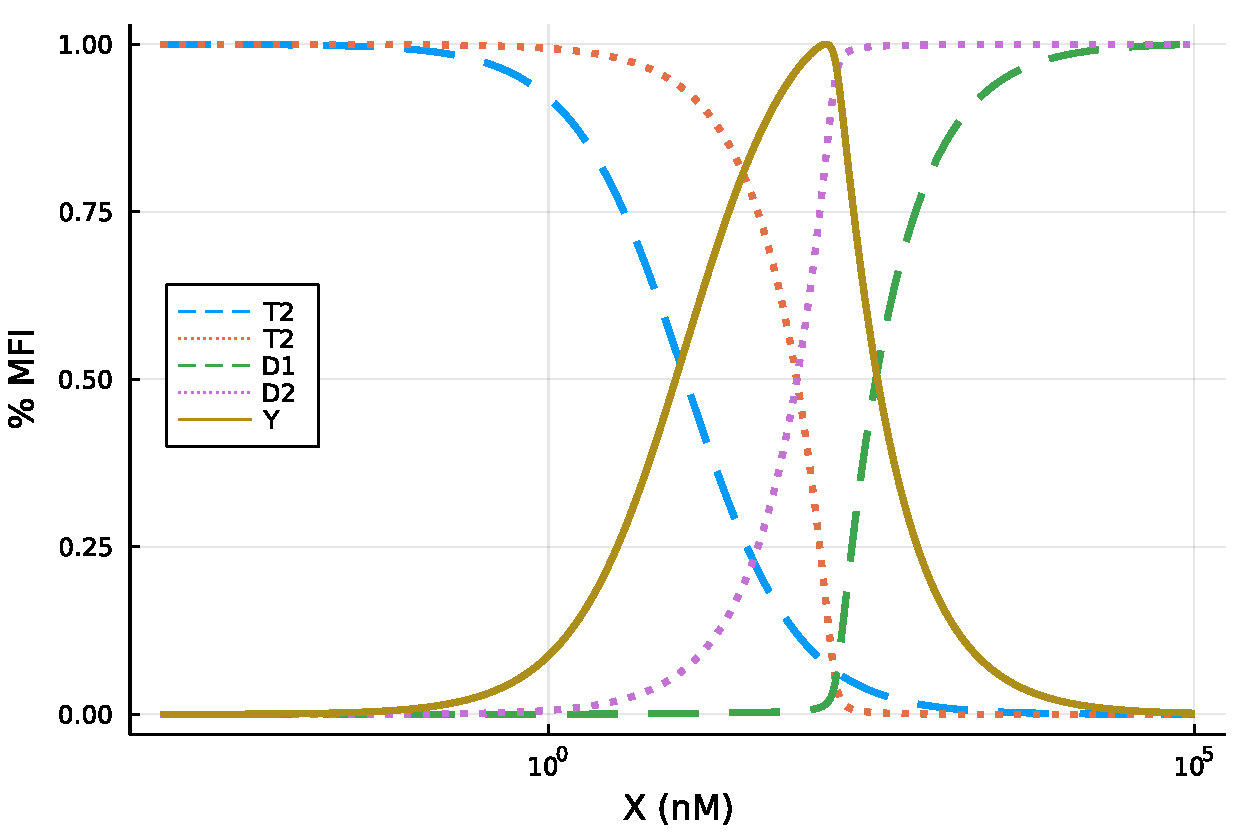
\includegraphics[width=1\textwidth]{fig/Dish_1.pdf}
		\caption{}
		\label{fig:3}
	\end{subfigure} 
	\begin{subfigure}[b]{0.49\textwidth}
		\centering
		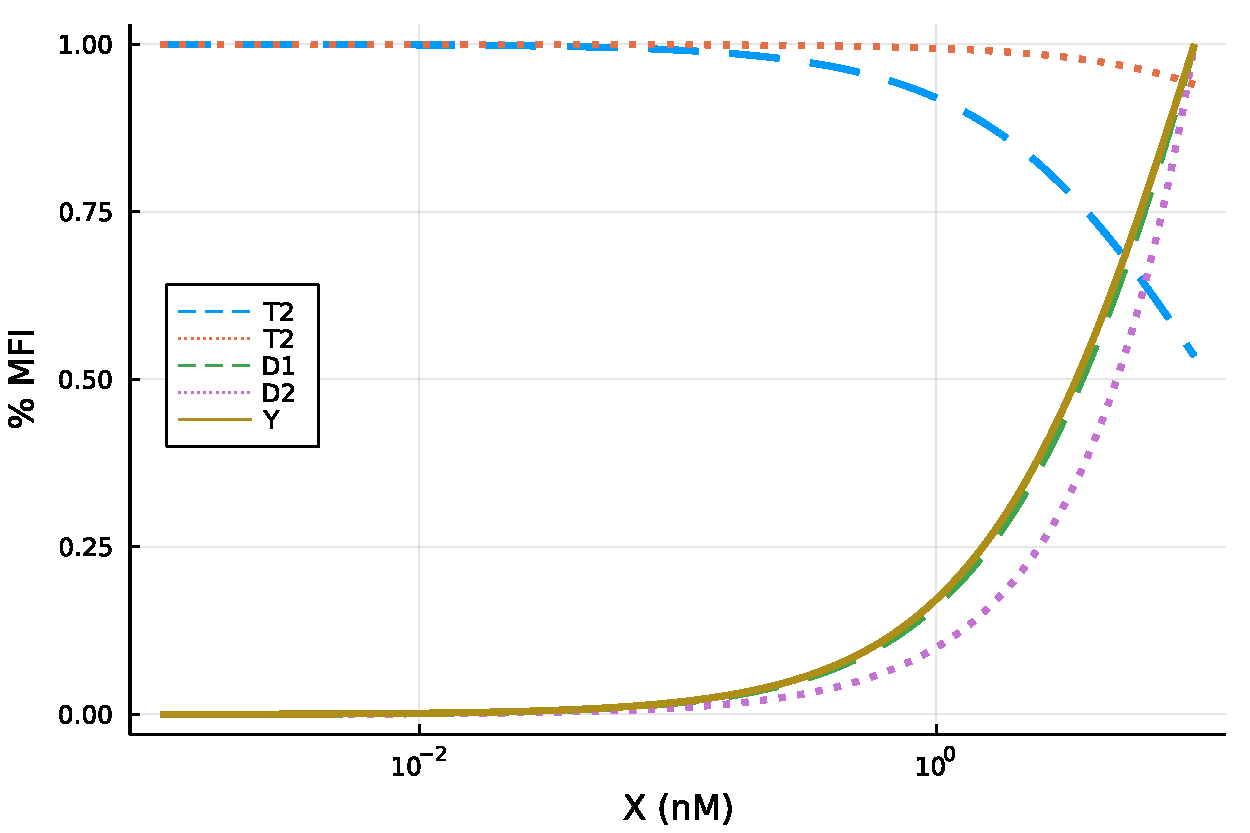
\includegraphics[width=1\textwidth]{fig/Dish_2.pdf}
		\caption{}
		\label{fig:4}
	\end{subfigure}
	\caption[Steady state simulations]{Steady state simulations of Model~\eqref{eq:three-body}. The vertical axis is the normalized to the \ac{MFI} levels of the variables in the experiments with different ranges of \ac{BiTE} antibody initial concentration. The initial \ac{BiTE} concentration range, range of horizontal axis values, in (a) is larger than (b). The plots on the left present the concentrations of the trimer and the targets, and the plots on the right side present the drug-target dimers concentrations.}
	\label{fig:ss}
\end{figure}

\section{Identifiability} \label{sec:identifiability}
The structural identifiability analysis of model~\eqref{eq:three-body} based on a given drug $X(t)$, the first target $T1(t)$ (immune cells receptor), and the second target $T2(t)$ (protein expressed on cancer cells) data is done. Results shows that all the parameters $k_{n1}$, $k_{f1}$, $k_{n2}$, and $k_{f2}$ are globally and locally identifiable. The computer software SIAN~\cite{hong2019sian}, structural identifiability was used to confirm this result. On the contrary, most experimental measurements are done at the steady state~\cite{dreier2002extremely,brischwein2006mt110,friedrich2012regression,root2016development,yeung2020optimized,mathur2020novel,giffin2021amg,deegen2021psma}. 

In the remainder of the identifiability analysis performed in this section, it is proved that the dissociation rates $k_{D1} = k_{f1}/k_{n1}$, and $k_{D2} = k_{f2}/k_{n2}$ are
identifiable for at most three steady state measurements. This result eliminates the need for extra measurements, e.g. surface resonance imaging, to determine the dissociation constants of BiTE
molecules.

\paragraph{In terms of state variables} 
Consider a steady state $X^*$, $T_1^*$, $T_2^*$, $D_1^*$, $D_2^*$, $Y^*$ of the system~\eqref{eq:three-body}. 
Then the numbers $X^*$, $T_1^*$, $T_2^*$, $D_1^*$, $D_2^*$, $Y^*$, and $k_{n1}$, $k_{n2}$, $k_{f1}$, $k_{f2}$ are related by a system of six polynomial equations obtained by setting the left-hand sides of~\eqref{eq:three-body} to zero. 
To compute the projection of its solution set to ($D_1^*$, $D_2^*$, $X^*$, $Y^*$, $k_{f1}$, $k_{f2}$)-coordinates (by performing elimination with Gr\"obner bases~\cite[Chapter 2, \S 1]{CLO}) and find that the projection satisfies the following equation:
\[
\left ( D_1^* k_{f1} + D_2^* k_{f2} + X^* k_{f1} + X^*k_{f2} \right )
\left ( D_1^*  D_2^* - X^* Y^* \right ) =0.
\]

Since the parameters and concentrations are positive, the left bracket does not vanish, so 
\begin{equation}\label{eq:stst1}
	X^* = \frac{D_1^* D_2^*}{Y^*}.
\end{equation}
Adding this relation to the original system of six equations and computing the projections to the ($D_1^*$, $D_2^*$, $Y^*$, $k_{f2}$, $k_{n2}$, $T_2^*$)- and ($D_1^*$, $D_2^*$, $Y^*$, $k_{f1}$, $k_{n1}$, $T_1^*$)-coordinates, respectively, it can be obtained that
\[
(D_1^* T_2^* k_{n_2} - Y^* k_{f_2}) (D_1^* - D_2^*) = 0, \quad \text{and}\quad (D_2^* T_1^* k_{n_1} - Y^* k_{f_1}) (D_1^* - D_2^*) = 0.
\]
For the generic case $D_1^* \neq D_2^*$, 
\begin{equation}\label{eq:stst2}
	T_1^* = k_{D_1} \frac{Y^*}{D_2^*},\quad \text{ and } \quad T_2^* = k_{D_2} \frac{Y^*}{D_1^*}.
\end{equation}

\paragraph{In terms of first integrals}
The system~\eqref{eq:three-body} has three conservation laws, due to the constraints on the initial conditions: $c_1=T_1(t) + D_1(t) + Y(t)$, $c_2 = T_2(t) + D_2(t) + Y(t)$, and $c_3 = X(t) + D_1(t) + D_2(t) + Y(t)$.
Based on the initial conditions, $c_3 = X(0)$.
To prove that for every positive values of $c_1, c_2, c_3$, there exists at most one positive steady state, we augment the system obtained by setting the right-hand sides of~\eqref{eq:three-body} to zero with equations 
\begin{equation}\label{eq:first_int_eq}
	c_1 - T_1^* - D_1^* - Y^* = c_2 - T_2^* - D_2^* - Y^* = c_3 - X^* - Y^* - D_1^* - D_2^* = 0.
\end{equation}
Given the obtained system of nine equations to compute the projections (again, using Gr\"obner bases) of the solution set to the $(A, c_1, c_2, c_3, k_{D1}, k_{D2})$-coordinates, where $A$ is taken to be $T_1^*$ or $T_2^*$, and find that these projections satisfy:
\begin{equation}\label{eq:via1int1}
	(T_1^*)^2 + (c_3 + k_{D1} - c_1)T_1^* - c_1 k_{D1} = 0 \quad \text{and}\quad(T_2^*)^2 + (c_3 + k_{D2} - c_2)T_2^* - c_2 k_{D2} = 0
\end{equation}
Consider the first equation as a quadratic equation in $T_1^*$. 
The product of the roots is equal to $-c_2k_{D2} < 0$, so at most one of the roots is real positive, so $T^*$ is uniquely determined.
The same applies to $T_1^*$.
Next, by computing projection to the ($D_2^*$, $T_1^*$, $T_2^*$, $c_1$, $c_2$, $c_3$, $k_{D1}$, $k_{D2}$)-coordinates, to find the following relation for $D_2^*$:
\begin{equation}\label{eq:via1int2}
	c_3 D_2^* + T_1^* T_2^* - c_2 T_1^* - c_1 T_2^* + c_3 T_2^* + c_1 c_2 - c_2 c_3 = 0,
\end{equation}
which implies that $D_2^*$ is uniquely determined.
Finally, $D_1^*, X^*,$ and $Y^*$ are uniquely determined using the following simple consequences of~\eqref{eq:first_int_eq}:
\begin{equation}\label{eq:via1int3}
	D_1^* - D_2^* + T_1^* - T_2^* - c_1 + c_2 = 0, \;\; Y^* + T_2^* + D_2^* - c_2 = 0,\text{ and } X^* + D_2^* - T_1^* + c_1 - c_3 = 0.
\end{equation}

\paragraph{Two experiments}
Assuming that three experiments were conducted as described above and the steady state data $(T_1^{[i]}, T_2^{[i]}, D^{[i]})$ is given for $i = 1, 2, 3$.
The identification approach is to consider the first two experiments.
Equations~\eqref{eq:stst1}, and~\eqref{eq:stst2} are used to write the following polynomial system:
\begin{subequations}
	\begin{align}
		Y^{[i]} X^{[i]} &= (c_1 - T_1^{[i]} - Y^{[i]}) (c_2 - T_2^{[i]} - Y^{[i]}), \\ 
		T_1^{[i]} X^{[i]} &= k_{D1} (c_1 - T_1^{[i]} - Y^{[i]}), \\ T_2^{[i]} X^{[i]} &= k_{D2} (c_2 - T_2^{[i]} - Y^{[i]}),\\ \text{ for }i &= 1, 2.
	\end{align}
\end{subequations}

To compute the projection of the solution set of this system to the ($k_{D1}$, $k_{D2}$, $T_1^{[1]}$, $T_1^{[2]}$, $T_2^{[1]}$, $T_2^{[2]}$, $X^{[1]}$, $X^{[2]}$)-coordinates (using Gr\"obner bases) and find relations of the form:
\begin{equation}\label{eq:alphas}
	A_1 k_{D1}^2 + A_2 k_{D1} + A_3 = 0,\quad \text{ and }\quad B_1 k_{D2} + B_2 k_{D1} + B_3 = 0,
\end{equation}
where $A_1$, $A_2$, $A_3$, $B_1$, $B_2$, $B_3$ are polynomials from $\mathbb{Q}[T_1^{[i]}, T_2^{[i]}, X^{[i]} \mid i = 1, 2]$.
Furthermore, $A_1$ and $B_1$ factor as follows:
\begin{subequations}
	\begin{align}
		A_1 &= X^{[1]} X^{[2]} (T_1^{[1]} X^{[2]} - T_1^{[2]} X^{[1]}) (T_1^{[1]} T_2^{[1]} X^{[2]} - T_1^{[2]} T_2^{[2]} X^{[1]}), \\ 
		B_1 &= T_1^{[1]} T_1^{[2]} (T_2^{[1]} X^{[2]} - T_2^{[2]} X^{[1]}).
	\end{align}
\end{subequations}
Therefore, $A_1$ and $B_1$ will not vanish as long as the ratios $\frac{X}{T_1}, \frac{X}{T_2}, \frac{X}{T_1 T_2}$ are different in the first two experiments.
Equations~\eqref{eq:via1int1}, \eqref{eq:via1int2}, and~\eqref{eq:via1int3} yield formulas for the steady state in terms of $k_{D1}, k_{D2}, c_1, c_2, c_3$.
These formulas are substituted in $\frac{X}{T_1}, \frac{X}{T_2}, \frac{X}{T_1 T_2}$ to obtain three non-constant functions with respect to $c_3$. Therefore, outside of a set of measure zero, $A_1$ and $B_1$ will not vanish. Thus, \eqref{eq:alphas} implies that generically, two experiments are sufficient to find $k_{D1}$ and $k_{D2}$ up to at most two options.

\paragraph{Three experiments}
For the three experiment case, since the projections above could be computed for the second and third experiment, not for the first and second, if  $T_1^{[1]}, T_2^{[1]}, X^{[1]}$ is substituted with $T_1^{[3]}, T_2^{[3]}, X^{[3]}$ in the first equation in~\eqref{eq:alphas}, there can be a true relation.
This will yield one more quadratic equation for $k_{D1}$, denoted by $\widetilde{A}_1 k_{D1}^2 + \widetilde{A}_2 k_{D1} + \widetilde{A}_3 = 0$.
If it is not proportional to the original equation, this will leave at most one value for $k_{D1}$. A sufficient condition for this non-proportionality would be $A_1 \widetilde{A}_3 - \widetilde{A}_1 A_3 = 0$. To check this, one can plug again the formulas of the steady state in terms of $k_{D_1}, k_{D_2}, c_1, c_2, c_3$ from~\eqref{eq:via1int1}, \eqref{eq:via1int2}, and~\eqref{eq:via1int3} and observe that $A_1 \widetilde{A}_3 - \widetilde{A}_1 A_3$ is a non-constant function in $k_{D1}$, $k_{D2}$, $c_1$, $c_2$, $c_3^{[1]}$, $c_3^{[2]}$, $c_3^{[3]}$. Therefore, $A_1 \widetilde{A}_3 - \widetilde{A}_1 A_3 \neq 0$ outside of a set of measure zero.Therefore, $k_{D_1}$ and $k_{D_2}$ are generically uniquely identifiable from three experiments.

\section{Optimal binding kinetics}

In this part we investigate the basic characteristics of the bell-shape response, trimer concentration presented in Figure~\ref{fig:3}, to have a better understanding of the optimal binding kinetics of a \ac{BiTE} antibody at the site of action, e.g. \ac{TME}. The maximum concentration of the trimer complex, peak of the bell shape, and its corresponding initial \ac{BiTE} antibody condition are taken as the main characteristic values of the bell-shape. The first step is to visualize the sensitivity of the peak of the bell-shape to the dissociation rates of the binding kinetics of the~\ac{BiTE} antibody to its targets, and target concentrations. The parameters used in this section are based on the model represented in~\cite{betts2019translational} for PF-06671008 \ac{BiTE} antibody for solid tumors.

Figure~\ref{fig:dish} represents how change of dissociation rates and initial concentration of the targets affect the peak of the trimer concentration, and its corresponding \ac{BiTE} antibody concentration. From the left side of figure~\ref{fig:5}, sensitivity of the maximum trimer peak to the dissociation rates, it can be observed that an increase in dissociation rates $k_{D1}$, and $k_{D2}$ significantly decrease the peak of the trimer concentration. On the other hand, by looking at the right side of figure~\ref{fig:5} it can be observed that the optimal concentration of \ac{BiTE} (the corresponding initial concentration of \ac{BiTE} antibody at the peak of the trimer concentration) will be decreased by reducing the $k_{D1}$ only, and increased by increasing either $k_{D1}$ or $k_{D2}$. This result demonstrates that higher affinity, i.e. lower value of the dissociation rates, of the \ac{BiTE} antibody is not effective in changing the maximum trimer concentration at the cite of action, i.g. in the \ac{TME}. The sensitivity of the maximum trimer concentration, and optimal~\ac{BiTE} antibody initial concentration to the initial concentrations of the targets on the immune cells $T_1(0)$, and cancer cells $T_2(0)$ is visualized in one dimensional plots of Figure~\ref{fig:6}. From the left side, it can be observed that the maximum trimer concentration is sensitive to $T1(0)$ and insensitive to $T2(0)$, which physically makes sense since the initial concentration of the first target, CD3 receptors on the immune system, is much less than the second target, P-cad protein on the tumor cells, in the \ac{TME}. This results is consistent with the sensitivity analysis presented by~\cite{betts2019translational}. Surprisingly, any change above 0.01x, or below 100x in the initial concentration of the target $T_1(0)$ is not effective in changing optimal \ac{BiTE} concentration, and significantly changes the optimal concentration \ac{BiTE} antibody.

The dissociation rates $k_{D1}$ and $k_{D2}$ are dependent on the design of the \ac{BiTE} antibody, while $T1(0)$ and $T2(0)$ are dependent on the tumor characteristics and variability among cancer patients. So, from the design perspective it would be ideal if the maximum trimer concentration and optimal \ac{BiTE} concentration be less sensitive to the initial concentration of the targets. From the toxicity perspective, it would be favorable if a lower concentration of \ac{BiTE} antibody can produce the same amount of trimer in the \ac{TME}. In the one dimensional analysis presented in figure~\ref{fig:5}, the optimal \ac{BiTE} can be decreased as the dissociation rate of the first target $k_{D1}$ becomes smaller, and it will result in a slightly higher trimer concentration that is favorable for efficacy.

\begin{figure}
	\centering
	\begin{subfigure}[b]{0.8\textwidth}
		\centering
		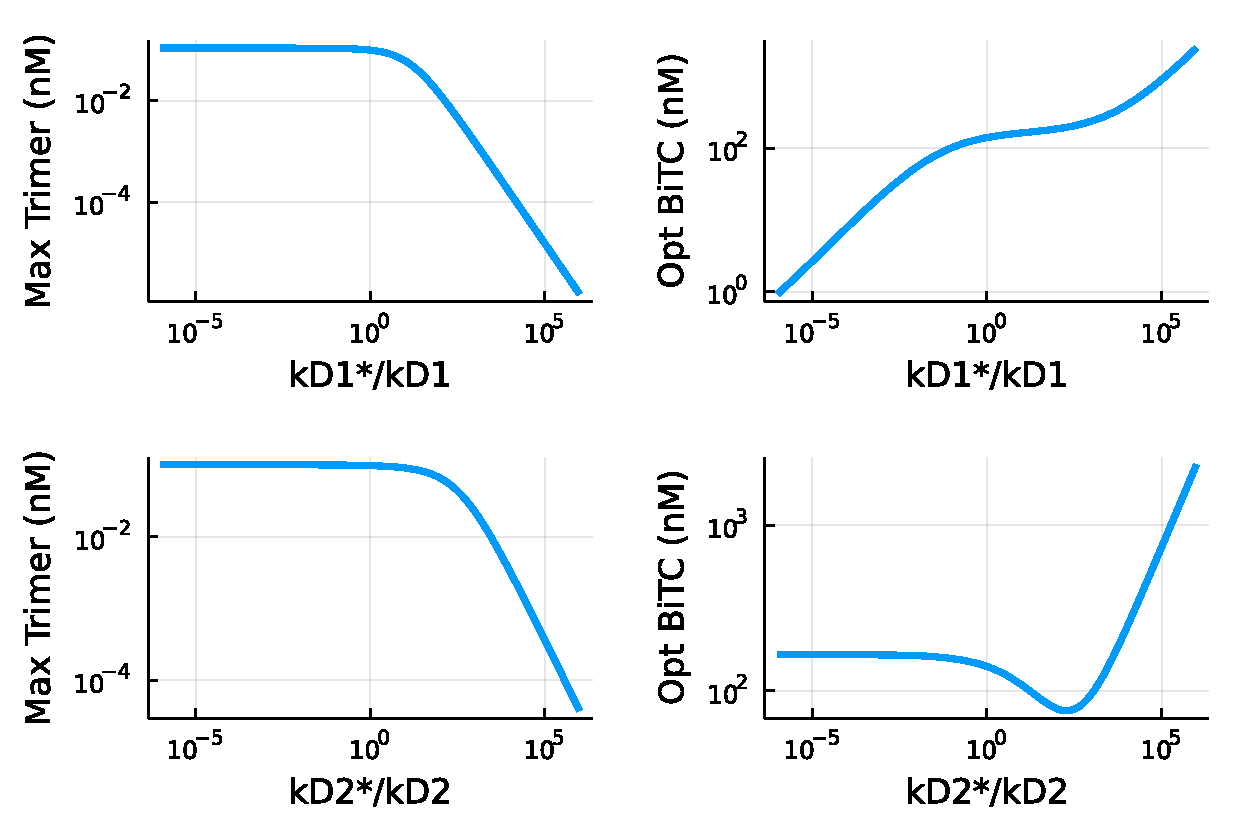
\includegraphics[width=1\textwidth]{fig/Dish_3.pdf}
		\caption{}
		\label{fig:5}
	\end{subfigure} \\
	\begin{subfigure}[b]{0.8\textwidth}
		\centering
		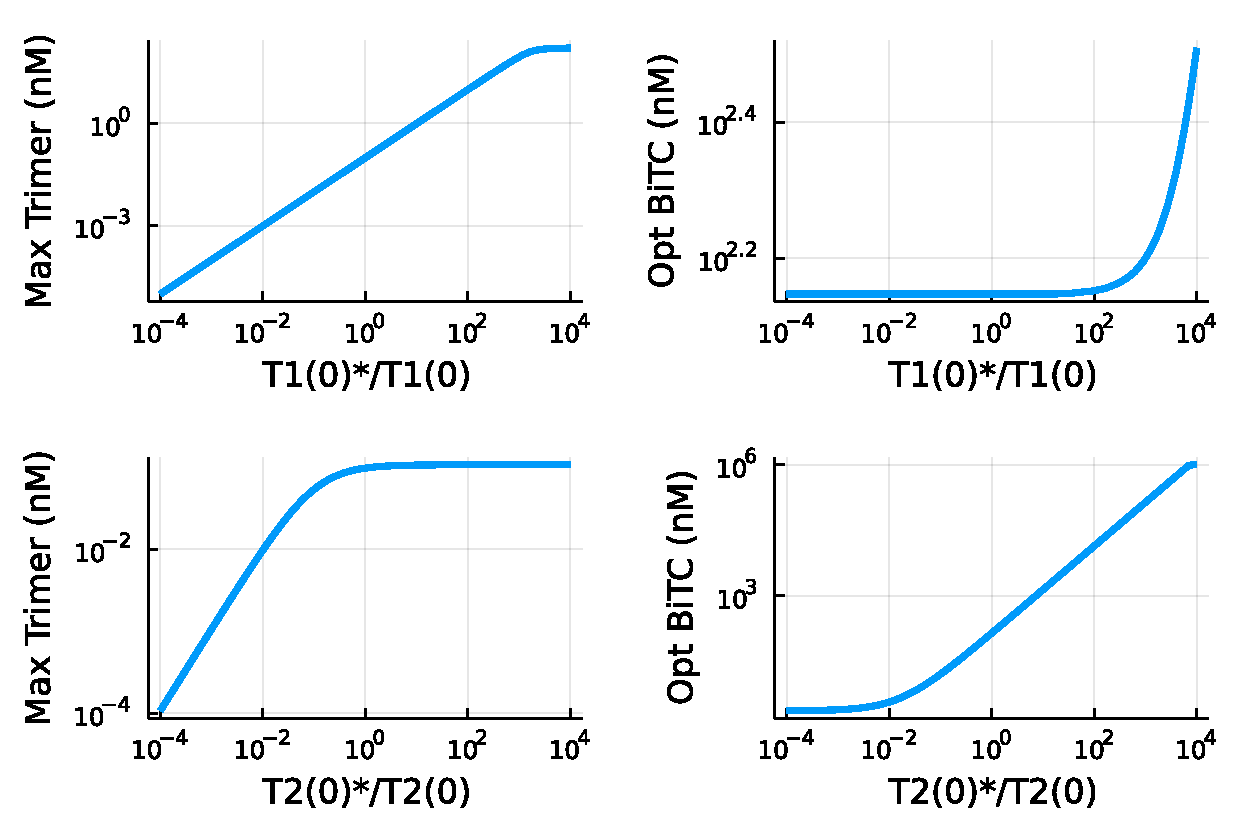
\includegraphics[width=1\textwidth]{fig/Dish_4.pdf}
		\caption{}
		\label{fig:6}
	\end{subfigure}
	\caption[Bell-shape characteristics]{Log-log plots of bell-shape characteristics: the effects of (a) sweeping \ac{BiTE} antibody dissociation rates to the targets and (b) sweeping target concentration in the \ac{TME} on the optimal concentration of trimer and \ac{BiTE}. The horizontal axes are log scale difference of the modified parameter (marked with a star*) and its original value. Maximum trimer concentration is the peak of the bell-shape, and Optimal \ac{BiTE} is the corresponding initial antibody concentration of the peak.}
	\label{fig:dish}
\end{figure}

\begin{figure}
	\centering
	\begin{subfigure}[b]{0.46\textwidth}
		\centering
		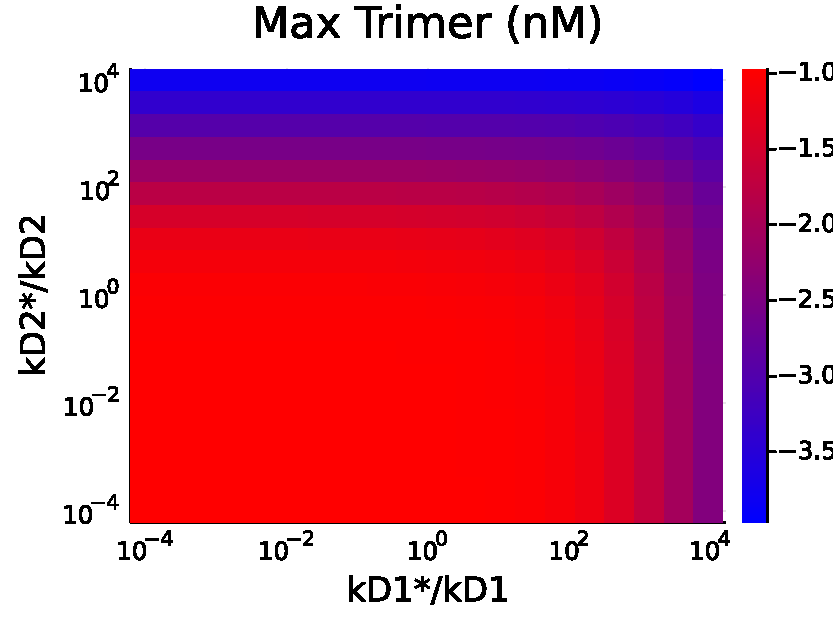
\includegraphics[width=1\textwidth]{fig/h1.pdf}
		\caption{}
		\label{fig:h1}
	\end{subfigure}
	\hspace{0.05\textwidth}
	\begin{subfigure}[b]{0.46\textwidth}
		\centering
		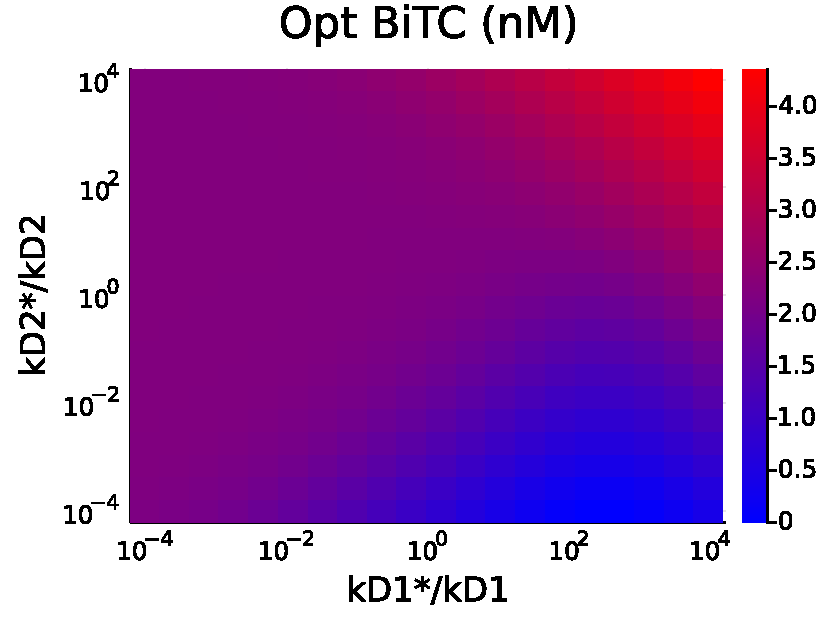
\includegraphics[width=1\textwidth]{fig/h2.pdf}
		\caption{}
		\label{fig:h2}
	\end{subfigure}
	\\
	\vspace{0.05\textwidth}
	\begin{subfigure}[b]{0.46\textwidth}
		\centering
		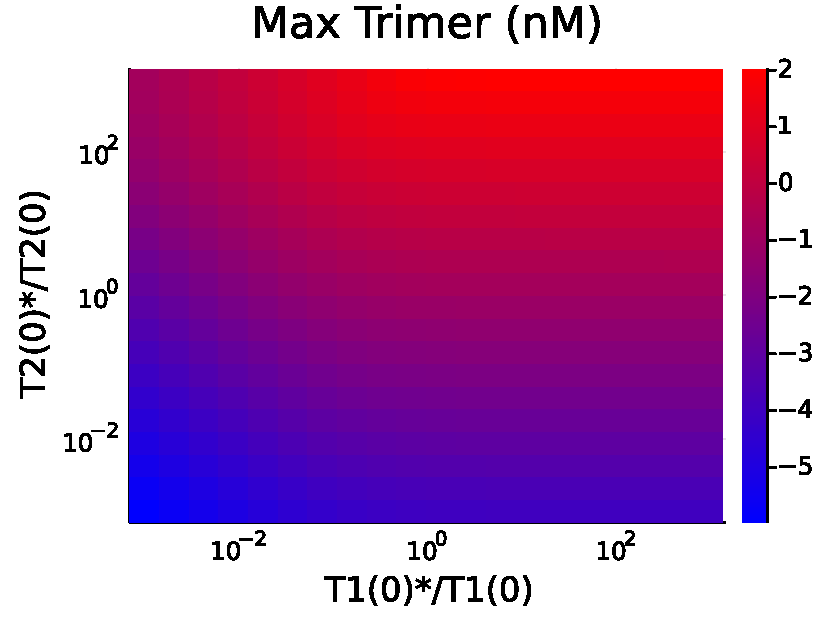
\includegraphics[width=1\textwidth]{fig/h3.pdf}
		\caption{}
		\label{fig:h3}
	\end{subfigure}
	\hspace{0.05\textwidth}
	\begin{subfigure}[b]{0.46\textwidth}
		\centering
		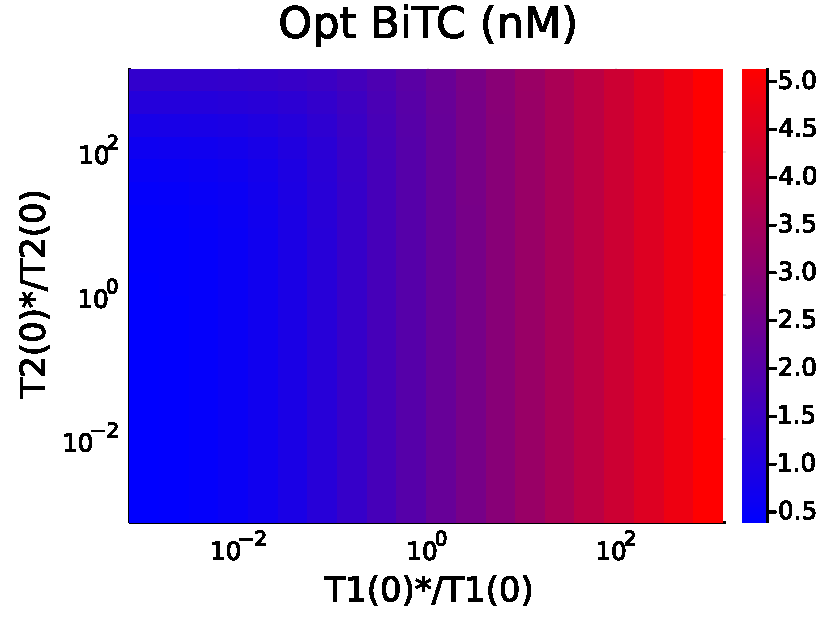
\includegraphics[width=1\textwidth]{fig/h4.pdf}
		\caption{}
		\label{fig:h4}
	\end{subfigure}
	\caption[Characteristics heatmap]{Bell-shape characteristics heatmap: the effects of sweeping the \ac{BiTE} antibody dissociation rates, $k_{D1}$ and $k_{D2}$, on (a) maximum of the trimer concentration of the bell-shape, and (b) corresponding, optimal, concentration of the \ac{BiTE} antibody are represented on top. The effect of sweeping initial target concentrations to (c) the peak of bell-shape, and (d) optimal concentration of the antibody are presented on the bottom. The colors are plotted in log scale concentrations in nM. The horizontal and vertical axes are in log scale difference of the modified parameter (marked with a star*) and its original value.}
	\label{fig:heat}
\end{figure}

Figure~\ref{fig:heat} extends the one dimensional visualizations presented in Figure~\ref{fig:dish} to two dimensions. The sensitivity of the maximum trimer concentration is on the left, and the sensitively of the corresponding initial concentration of the~\ac{BiTE} antibody is on the right side. The red color represents a higher value of the nM concentrations in log scale, and the blue color represents lower concentrations. The vertical pattern in Figure~\ref{fig:h1}, and the horizontal pattern in Figure~\ref{fig:h4} are consistent with the conclusions made from Figure~\ref{fig:dish}. Moreover, the contrasting colors in the top left and the bottom right of Figure~\ref{fig:h2} suggest that a simultaneous increase in dissociation rates $k_{D1}$, with a decrease in $k_{D2}$ is favorable in reducing the required concentration of \ac{BiTE} antibody to achieved the peak of the trimer concentration. A cross check between Figures~\ref{fig:h1}, and~\ref{fig:h2} indicates that the simultaneous changes in $k_{D1}$, and $k_{D2}$ to reduce the required trimer concentration to achieve the maximum concentration might not be favorable in increasing the maximum trimer concentration at the~\ac{TME}.

\section{Comparison between~\ac{BiTE} antibodies}

The presented three-body model~\ref{eq:three-body} is used here to have a quantitative measure in comparing different CD3 \ac{BiTE} antibody molecules presented in Table~\ref{table:bites}. The antibody molecules included in this study are designed for the two general categories of solid, and liquid tumors. Although each of the molecules might be different in the distribution, metabolism, and pharmacokinetics characteristics, the three-body model is what they all have in common at the cite of action. Beside the dissociation constants $k_D$ values presented in Table~\ref{table:bites}, the initial concentration of the targets is necessary for computational simulations of the three-body model. As the initial concentration of the target receptors is highly dependent of the cancer type and it might vary across different regions of the tumor, the comparison between the bell-shapes of \ac{BiTE} molecules should be done for different initial concentrations of the targets.

A visual comparison between the bell-shapes of the molecules considered in this study is presented in Figure~\ref{fig:res1}. The ratio of the initial concentration of the targets ($T_1(0):T_2(0)$) are considered to be in the range of 1:10 to 1:1000 for solid tumors (Figure~\ref{fig:7}), and in the range of 10:1 to 1:10 for liquid tumors (Figure~\ref{fig:8}). It can be observed that in addition to the peak of the bell-shape, and the corresponding concentration of the \ac{BiTE} antibody, the width of the bell-shape varies at different ratio of the initial concentration of the targets. For instance the width of the \ac{BiTE} antibody Tarlatamab increases for dense tumor, where the initial concentration of the target proteins on cancer cells is much more than the target proteins on immune cells. 

An analytic formulation of the basic characteristics of the bell-shape is done by~\cite{douglass2013comprehensive}. The theoretical analysis has been done to understand the sensitivity of the peak of the bell-shape to binding kinetics of the bispecific antibody to each of the targets. Moreover, the with of the bell-shape could be approximated by initial concentrations of the targets at the cite of action. The presented results in this study is to have a quantitative comparisons between the \ac{BiTE} molecules. For more theoretical understanding of the three-body problem, the readers are encouraged to the supplementary materials of~\cite{douglass2013comprehensive}.

The quantitative framework used for comparing bell-shapes of the \ac{BiTE} antibody molecules at different ratios of initial concentration of the targets can be extended to continuous ratios of the targets. For this purpose, the basic characteristics of the bell-shape are extracted across different ratios between the targets, and represented in Figure~\ref{fig:res2}. The peak of the trimer concentration is the maximum of bell-shape (on top), the corresponding \ac{BiTE} concentration is the initial concentration of \ac{BiTE} antibody that results in the maximum of the bell-shape (on middle), and the bell-shape width is simply the range of the \ac{BiTE} antibody concentration that results in at least 50\% of the maximum of the bell-shape (on bottom). For a realistic comparison between the \ac{BiTE} antibodies design for solid tumors (Figure~\ref{fig:9}), the left hand side of the horizontal axis should be considered, where the initial concentration of the target protein on cancer cells is much more that the initial concentration of the target protein CD3 on immune T cells. Similarly, for a realistic comparison between the \ac{BiTE} antibodies designed for liquid tumors (Figure~\ref{fig:10}), the right middle or right side of the horizontal should be taken into consideration.

\begin{figure}
	\centering
	\begin{subfigure}[b]{0.48\textwidth}
		\centering
		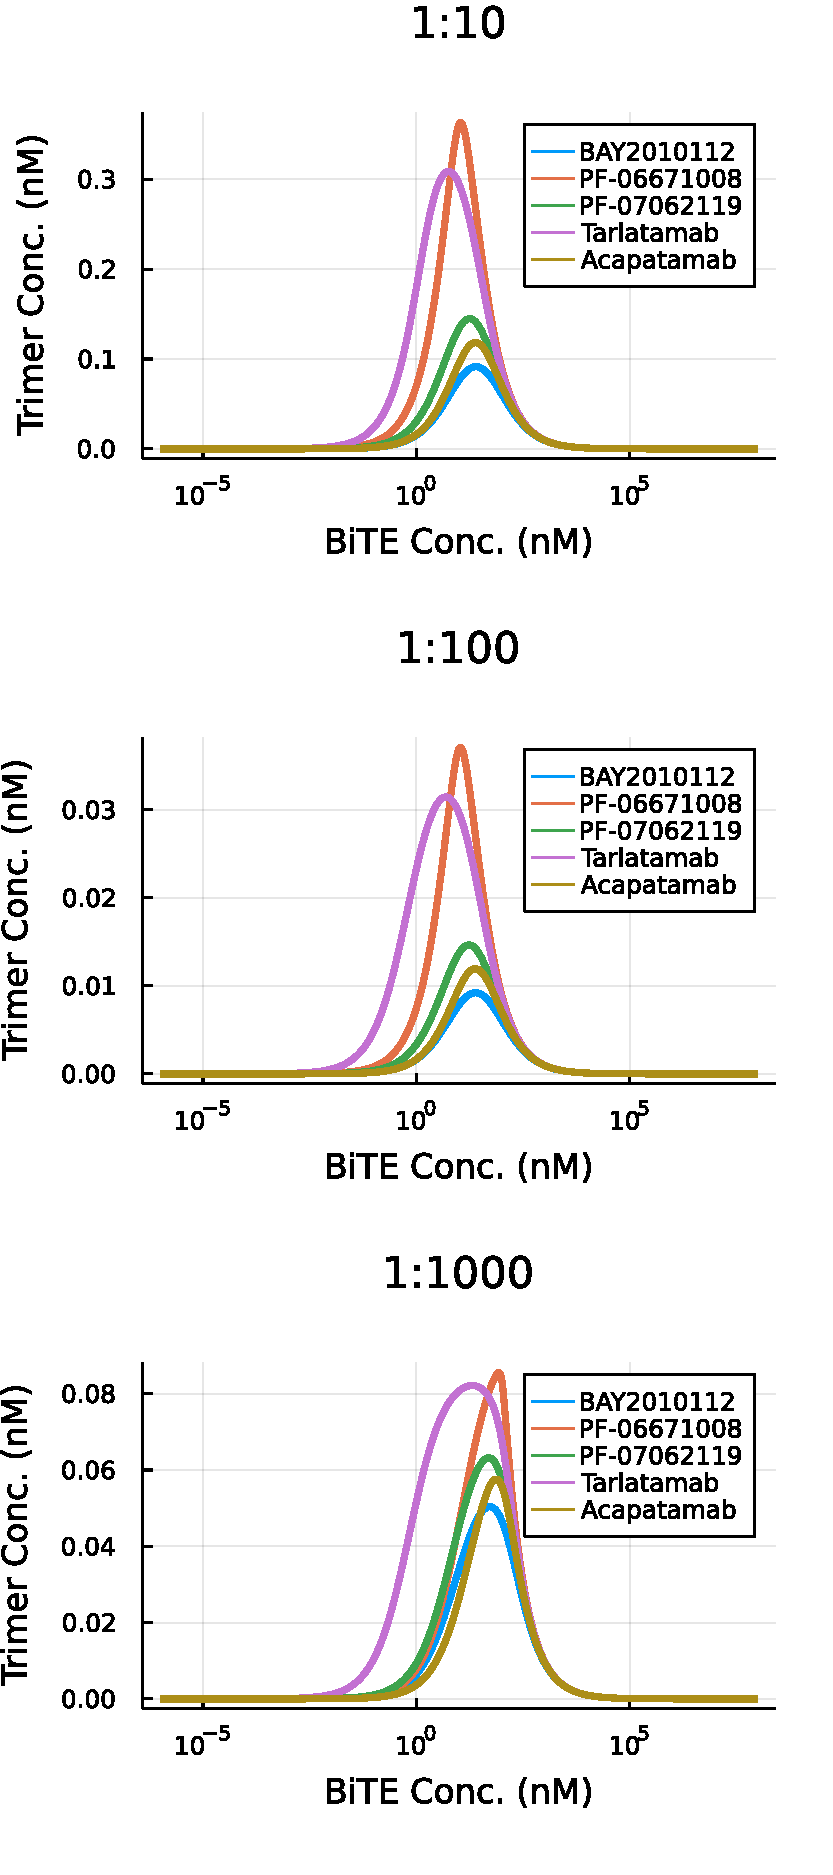
\includegraphics[width=1\textwidth]{fig/solid.pdf}
		\caption{}
		\label{fig:7}
	\end{subfigure} 
	\begin{subfigure}[b]{0.48\textwidth}
		\centering
		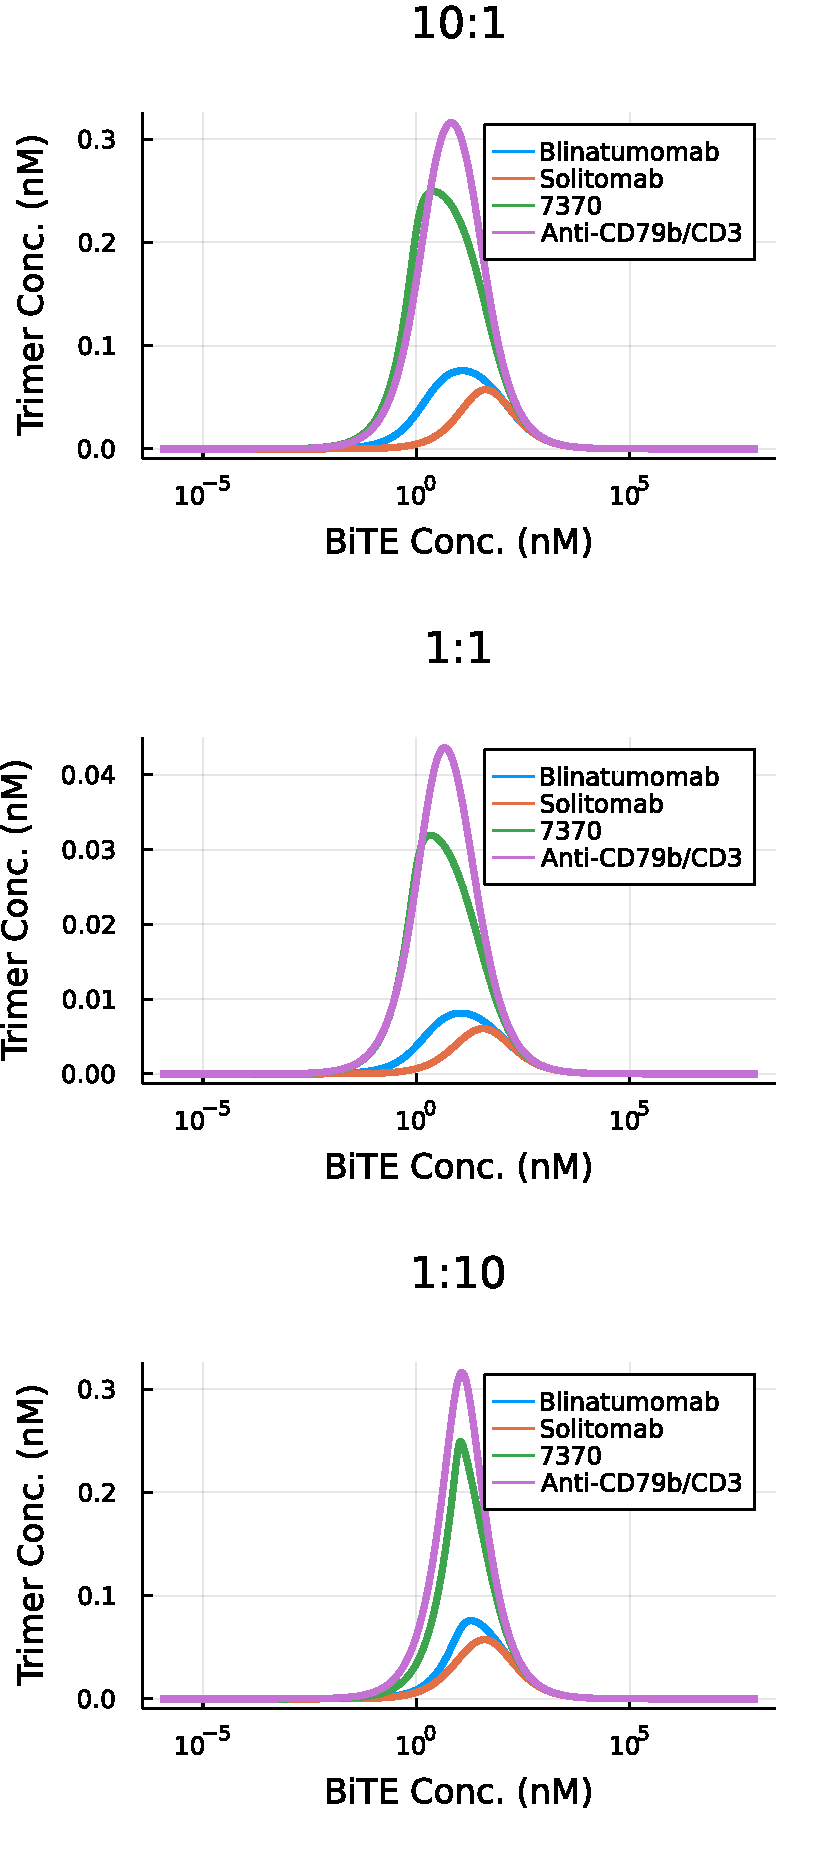
\includegraphics[width=1\textwidth]{fig/liquid.pdf}
		\caption{}
		\label{fig:8}
	\end{subfigure}
	\caption[Comparison of bell-shapes]{Numerical comparison between the bell shapes of \ac{BiTE}s designed for (a) solid, and (b) liquid tumors. The relative concentration of the targets $T_1(0):T_2(0)$ is printed on the top of each plot. The horizontal axes are in log scale, and the vertical axes are in linear scale.} 
	\label{fig:res1}
\end{figure}

\begin{figure}
	\centering
	\begin{subfigure}[b]{0.48\textwidth}
		\centering
		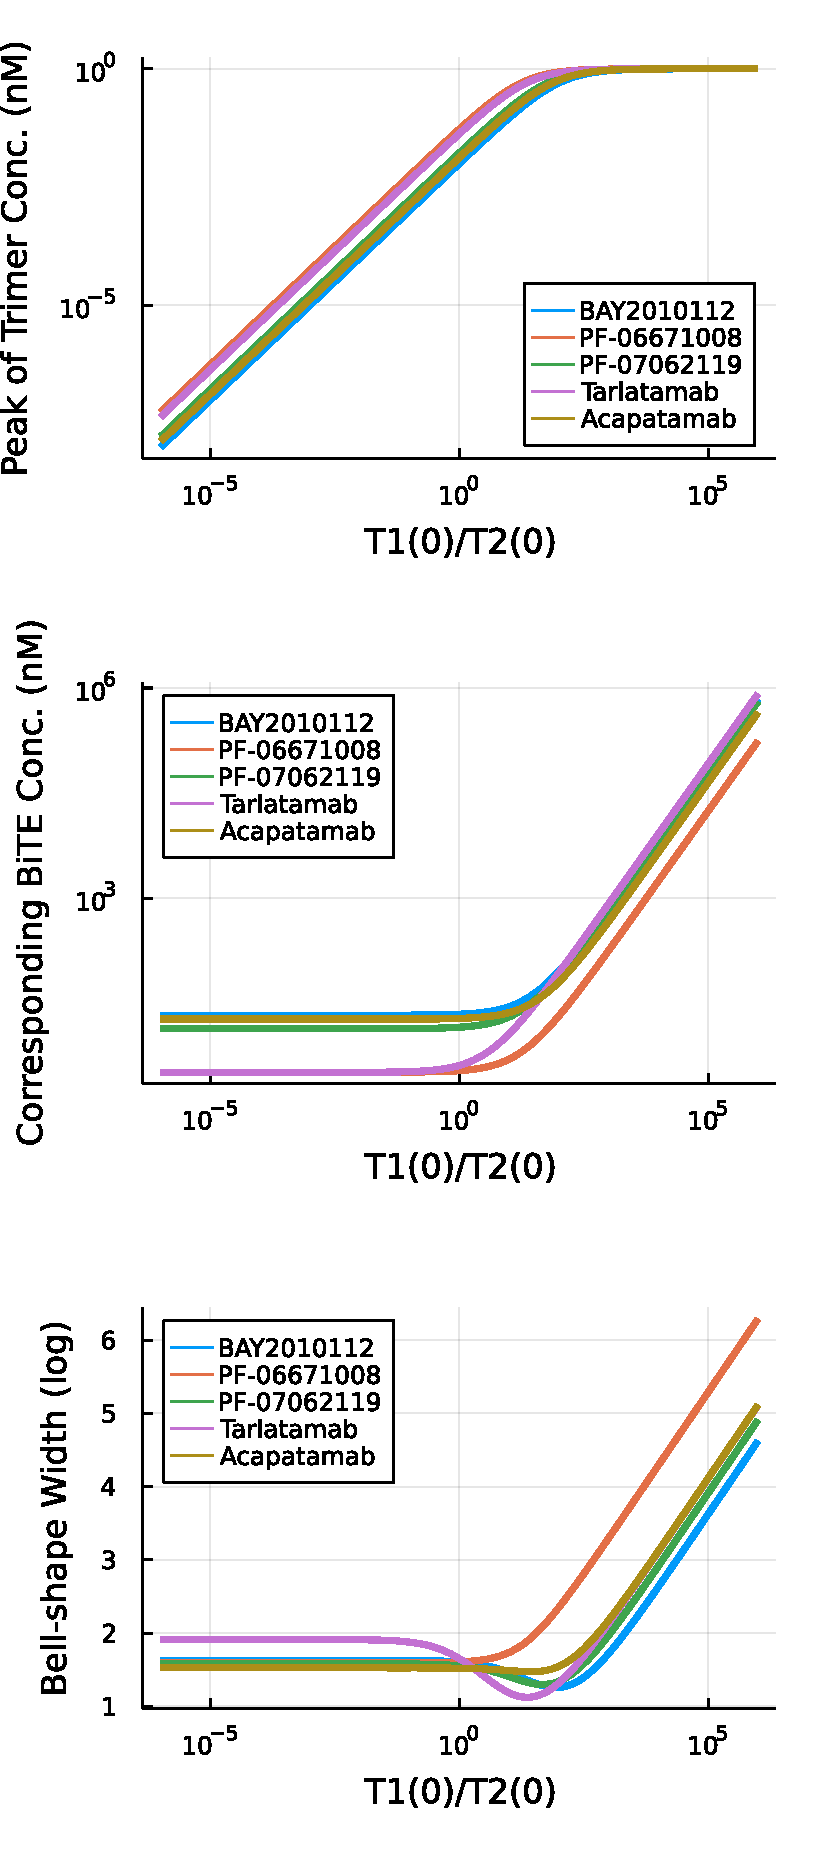
\includegraphics[width=1\textwidth]{fig/compare-solid.pdf}
		\caption{}
		\label{fig:9}
	\end{subfigure} 
	\begin{subfigure}[b]{0.48\textwidth}
		\centering
		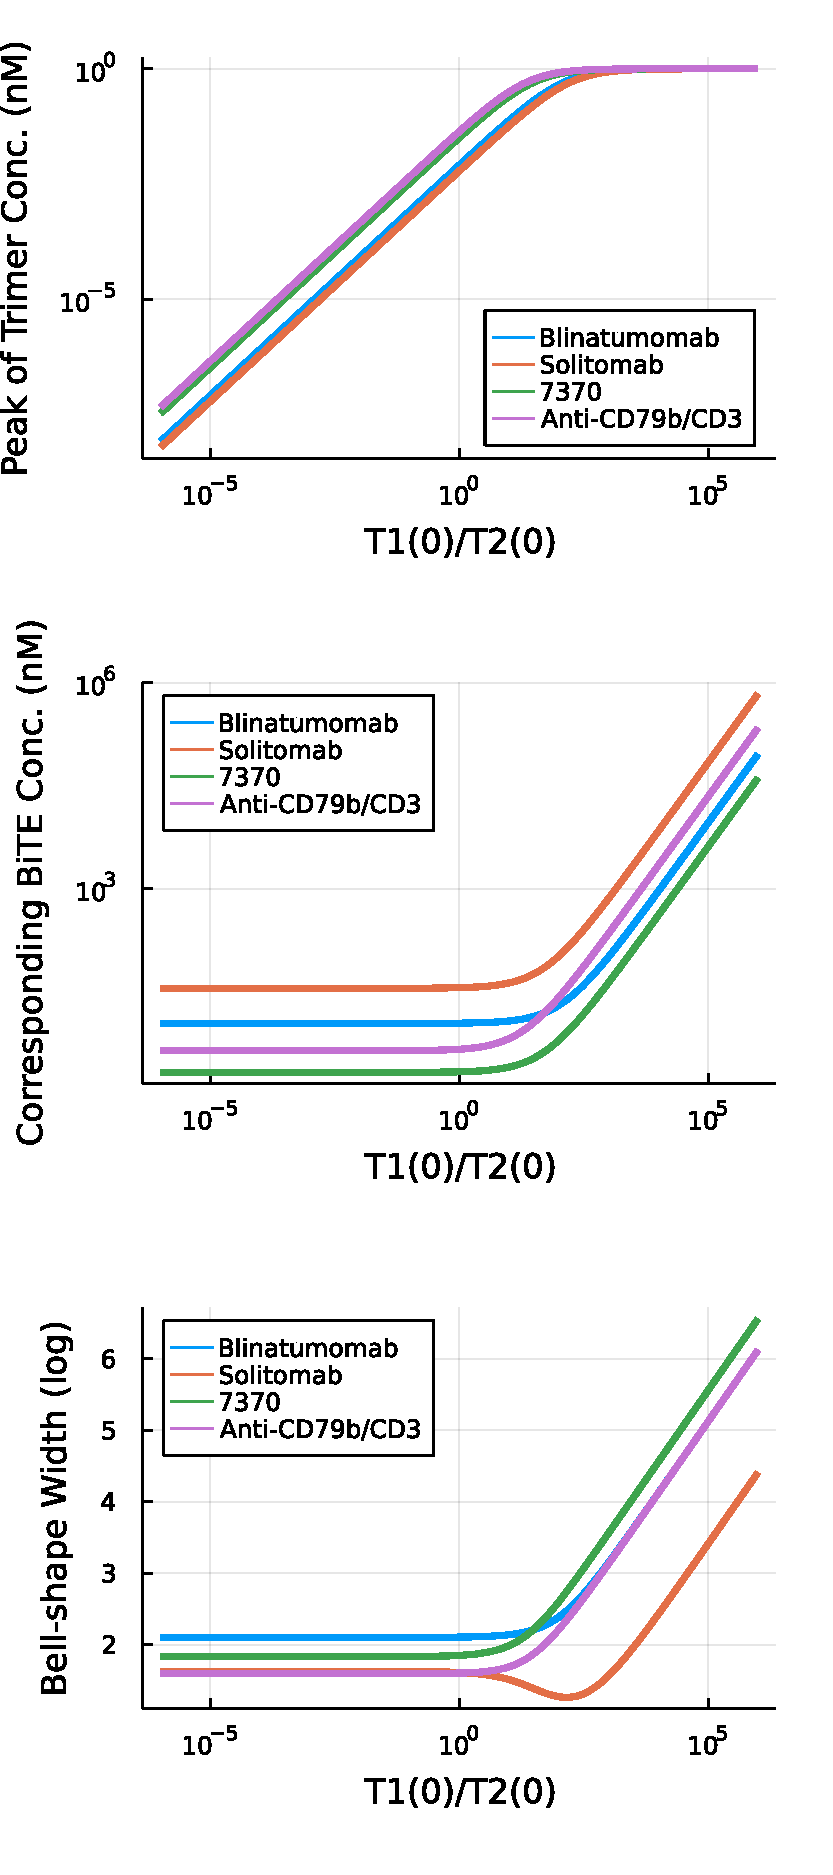
\includegraphics[width=1\textwidth]{fig/compare-liquid.pdf}
		\caption{}
		\label{fig:10}
	\end{subfigure}
	\caption[Comparison of the characteristics of the bell-shapes]{Numerical comparison between the basic characteristics of the bell-shape response of different \ac{BiTE}s designed for (a) solid, and (b) liquid tumors. The top figure represent the value of the peak of bell-shape, the middle figures represent the corresponding \ac{BiTE} antibody concentration at the peak of the bell-shape, and the bottom figures represent the width of the peak of the bell-shape. The relative initial concentration of the targets $T_1(0)/T_2(0)$ is visualized in log scale of the horizontal axes.} 
	\label{fig:res2}
\end{figure}

From the three-body model perspective, a promising \ac{BiTE} antibody is the one that creates the most trimer concentration with the minimal initial concentration of the antibody at the cite of action. Also, to overcome natural variability among different cancers and patients it is favorable to have a \ac{BiTE} antibody with minimal variation for different ratios of the initial concentrations of the targets. So, A \ac{BiTE} antibody molecule is effective at the cite of action if it results in: 1) a relatively higher peak of the trimer concentration, 2) a lower corresponding concentration of the \ac{BiTE} at the peak of the trimer concentration, 3) a larger width of the bell-shape. Among the molecules presented in Figure~\ref{fig:res2}, it can be observed the \ac{BiTE} molecules like 7370, and PF-06671008 are outperforming in creating a large concentration of trimer concentration of tumor with minimal initial concentration. On the other hand, \ac{BiTE}antibody molecule Solitomab, is creating a stable width of the peak for a wide range of ratios between the initial concentrations of the targets. It is apparent that, stability across different initial concentration of the targets increases the consistency of the data in clinical research.

\section{Bio-distribution}
A full dynamic model for \ac{BiTE} for in human for \ac{IV} dose is introduced in~\cite{betts2019translational}. A slightly different version of this model is used here as an starting point.

\begin{subequations} \label{eq:full}
	\begin{align}
		\dot{X_c} &  = \rho u(t) - k_{elD} X_c - k_{cp} X_c + k_{pc} X_p \frac{V_p}{V_c} - k_{cl} X_c  - k_{lc} X_l \frac{V_l}{V_c} \nonumber \\ &\qquad - k_{n1} X_c T1_c + k_{f1} D1_c  - k_{n2} C_c T2_c + k_{f2} D2_c - k_{td} (X_c-\frac{X_t}{k_\varepsilon}) \frac{X_1+X_2}{w V_c} ,\\
		\dot{X_p} &  = k_{cp} X_c \frac{V_c}{V_p} - k_{pc} X_p,\\
		\dot{X_l} &  = k_{cl} X_c \frac{V_c}{V_l} - k_{lc} X_l,\\
		\dot{T1_c} &= - k_{ctT} T1_c + k_{tcT} T1_t \frac{M_1 +M_2}{w V_c} -k_{n1} X_c T1_c -k_{f1} D1_c, \\
		\dot{D1_c} &= k_{n1} X_c T1_c -k_{f1} D1_c, \\
		\dot{T2_c} &= k_{syn} - k_{deg} T2_c - k_{n2} X_c T2_c + k_{f2} D2_c, \\
		\dot{D2_c} &= -k_{elD}*D2_c +k_{n2} X_c T2_c -k_{f2} D2_c,\\
		\dot{X_t} &  = k_{td} (X_c-\frac{X_t}{k_\varepsilon}) - k_{n1} T1_t X_t - k_{n2} T2_t X_t + k_{f1} D1_t + k_{f2} D2_t,\\
		\dot{T1_t} & = k_{ctT} T1_c \frac{w V_c}{M_1+M_2} - k_{tcT} T1_t - k_{n1} T1_t C_t + k_{f1} D1_t - k_{n1} T1_t D2_t + k_{f1} Y,\\
		\dot{T2_t} & = - k_{n2} T2_t C_t + k_{f2} D2_t - k_{n2} T2_t D1_t + k_{f2} Y,\\
		\dot{D1_c} & = k_{n1} C_c T1_c - k_{f1} D1_c\\
		\dot{D1_t} & = k_{n1} T1_t C_t - k_{f1} D1_t - k_{n2} T2_t D1_t + k_{f2} Y ,\\
		\dot{D2_t} & = k_{n2} T2_t C_t + k_{f2} D2_t - k_{n1} T1_t D2_t + k_{f1} Y,\\
		\dot{Y} & = k_{n1} T1_t D2_t + k_{n2} T2_t D1_t - (k_{f1}+k_{f2}) Y, \\
		\dot{M_1} & = \frac{k_{ge} M_1 (1-\frac{M_1+M_2}{k_{v}})}{(1+(\frac{k_{ge}}{k_{gl}} (M_1+M_2))^{k_\psi})^{1/k_\psi}} -\frac{k_{max}\times Y}{kc_{50}+Y} M_1, \\
		\dot{M_2} & = \frac{k_{max}\times Y}{kc_{50}+Y} M_1 - M_2/k_\tau.
	\end{align}
\end{subequations}
% 
Where $X$ is the concentration of drug, $T$ is the concentration of targets, $D$ is the drug-target dimer concentration, $Y$ is the trimer concentration, and $M$ is the tumor volume intermediate compartment. 
All parameters and variables are defined in details in tables \ref{table:def1} and \ref{table:def2}. 
The dot sign on top of the variables is a time derivative $\dot{f}(t)=\frac{df(t)}{dt}$. 
The differences between model~\ref{eq:full} and the model presented in~\cite{betts2019translational} are: 1) an extra medium for representing tissues with high concentration of immune cells, e.g. lymph nodes, 2) integrating tumor intermediate compartments into the other modules of the model, and 3) lower number of tumor intermediate compartments for representing the delay.
%
\begin{landscape}
	\begin{table}[!ht]
		\centering
		\caption{Parameters used in model~\eqref{eq:full}.}
		\begin{tabular}{c l  l  l} 
			\hline
			& Value & Unit & Definition \\ [0.5ex] 
			\hline\hline
			$V_{c}$ & $40.2$ & mL/kg & Volume of distribution in the central compartment \\ 
			$V_{p}$ & $211$ & mL/kg & Volume of distribution in the peripheral compartment  \\ 
			$V_{l}$ & $92$ & mL/kg & Volume of distribution in the lymph compartment  \\ 
			$k_{el_D}$ & $1.16\times10^{-1}$ & 1/h & Elimination rate of antibody in the central compartment \\ 
			$k_{el_T}$ & $2.51$ & 1/day & Elimination rate of immune cells (Target 1)  \\ 
			$k_{cp_D}$ & $6.27\times10^{-1}$ & 1/h & Antibody redistribution to the peripheral compartment \\ 
			$k_{pc_D}$ & $1.19\times10^{-1}$ & 1/h & Antibody redistribution to the central compartment \\
			$k_{ct_T}$ & $2\times10^{-3}$ & 1/day & T cell (target 1) redistribution to the \ac{TME} \\ 
			$k_{tc_T}$ & $5\times10^{-4}$ & 1/day & T cell (target 1) redistribution to the central compartment\\ 
			$k_{n_1}$ & 1.72& 1/nM/h& Binding of the antibody and target 1 \\ 
			$k_{f_1}$ & 19.66& 1/h& Unbinding rate of the antibody-target 2 dimer \\ 
			$k_{n_2}$ & 1.57& 1/nM/h & Binding rate of the antibody and target 2 \\ 
			$k_{f_2}$ & 0.74 & 1/h & Unbinding rate of the antibody-target 2 dimer \\ 
			$k_{deg}$ & $1.5\times 10^{-1}$ & 1/h & Tumor $T2_c$ degradation rate \\
			$k_{syn}$ & $k_{deg} \times T2_c(0)$ & 1/h & Tumor synthesis rate (assuming no proliferating tumor) \\
			$k_{ctT}$ & $2 \times 10^{-3}$ & 1/day & T cell redistribution from the central to the \ac{TME} \\
			$k_{tcT}$ & $5\times 10^{-4}$& 1/day & T cell redistribution from the \ac{TME}.  \\
			$k_{max}$ & 1.32& 1/day & Maximum killing rate  \\
			$kc_{50}$ & $6.9\times 10^{-5}$& nM & Concentration at half maximum  \\
			$k_{ge}$ & $1.9\times 10^{-1}$& 1/day & Exponential tumor growth rate  \\
			$k_{gl}$ & $1.23 \times 10^{-1}$& mL/day & Linear tumor growth rate  \\
			$k_{v}$ & $6.0$& mL & Maximum tumor volume  \\
			$k_{\tau}$ & 3.99& day& Transduction time between tumor compartments.  \\
			$k_{\psi}$ & 20 & 1 & Exponential to linear transition rate of the tumor  \\
			$w$ & 60 & kg & Weight of a patient.  \\
			$\rho$ & 9.52 & nM/($\mu\text{g}$/kg) & Drug conc. in the central compartment for $1\mu\text{g}$/kg dose  \\[1ex] 
			\hline
		\end{tabular}
		\label{table:def1}
%		\caption*{The tumor growth rate parameters are based on mouse experiments done with HCT116 cell line along with T cell adoptive transfer tumor model, reported by \cite{betts2019translational}.}
	\end{table}
	
	
	\begin{table}[ht!]
		\centering
		\caption{Variables used in model~\eqref{eq:full}.}
		\begin{tabular}{c  l  l  l  l} 
			\hline
			Variable & Unit & Initial value &Definition \\ [0.5ex] 
			\hline
			$u$ & mg/kg/day & - & Input: drug dose.\\
			$X_c$ & nM & 0.0 & Antibody concentration in central compartment. \\ 
			$X_p$ & nM & 0.0 & Antibody concentrations in peripheral compartment. \\
			$X_t$ & nM & 0.0 & Antibody concentrations in the \ac{TME}.\\
			$T1_c$ & nM & 0.83 & Target 1 concentration in the central compartment. \\ 
			$T1_t$ & nM & $1.08 \times 10^{-1}$ & Target 1 concentration in the \ac{TME}. \\
			$T2_c$ & nM & 1.1 & Target 2 concentration in the central compartment.\\
			$T2_t$ & nM & $1.66\times 10^2$& Target 2 concentration in the \ac{TME}.\\
			$D1_c$ & nM & 0.0 & Dimer drug-target 1 in the central compartment. \\ 
			$D1_t$ & nM & 0.0 & Dimer drug-target 1 in the \ac{TME}. \\
			$D2_c$ & nM & 0.0 & Dimer drug-target 2 in the central compartment.\\
			$D2_t$ & nM & 0.0 & Dimer drug-target 2 in the \ac{TME}.\\
			$Y$ & nM & 0.0 & Trimer concentration in the \ac{TME}. \\
			$M1$ & mL & 1.0 & Tumor volume in growth compartment. \\
			$M2$ & mL & 0.0 & Tumor transduction compartment. \\[1ex] 
			\hline
		\end{tabular}
		\label{table:def2}
	\end{table}
\end{landscape}


\section*{Computational resources}
SIAN~\cite{hong2019sian} is used for structural identifiability analysis, and analytical derivations. Numerical simulations and figures are produced with Julia programming language~\cite{Julia-2017}. DifferentialEquations package is used numerical calculations~\cite{DifferentialEquations.jl-2017}. The numerical software for reproducing the figures presented in the manuscript along with more examples is available at \url{https://github.com/mahdiarsadeghi/bites}.

\section*{Acknowledgment}
This chapter could never be completed without the help of Irina Kareva, Gleb Pogudin, and Anup Zutshi. The discussions with Kumpal Madrasi and Abed Alnaif increased the value of this study.